A Soft Error or Single Event Upset is a random, non-catastrophic error, where radiation causes
a perturbation to a circuit by temporarily altering a single signal or datum.
Detecting and mitigating such errors is highly important in some fields, such as satellite design, 
where high design costs, harsh environments, and difficulties to repair once deployed make it necessary. 
However with the continuing increasing of semiconductor densities the current soft error
challenges experienced in space will likely be future problems for terrestrial devices\cite{normand1996single}\cite{henkel2013reliable}.

FPGA devices work through mapping circuit descriptions into a collection of Logic Blocks,
which are described in programmable look-up-tables and routed together via
programmable switchboxes.
Configuration data for both the look-up-tables and switchboxes are stored in a
configuration memory, which means soft errors can either change the functionality
of Logic Blocks or can change the routing between them.
Other memories called Block memory and flip-flops are also present in FPGA devices,
and soft errors in these regions can alter the state of the circuit but not the
circuits functionality.

%How this changes the protection strategy compared to software and VLSI
For VLSI/ASIC designs registers are the most vulnerable to soft-errors, with
combinational logic contributing very little \cite{baumann2005soft} this makes
approaches which asses and protect vulnerable registers promising \cite{chen2014reliability}.
However in FPGA devices the most vulnerable region is the configuration memory
so such approaches would have little impact requiring alternative methods.

%ECC and frame based checking approaches
Circuits described within configuration memory are usually protected in one of two ways,
either the circuit is replicated with comparison, or ECC/CRC signals associated with
frames of the configuration memory are scanned for errors.
Replication uses extra area and power however error detection latency is low,
while ECC/CRC checks consume less area and power but detection latency is higher and
it is limited to only protecting configuration memory.

\begin{figure}[h]
\centering
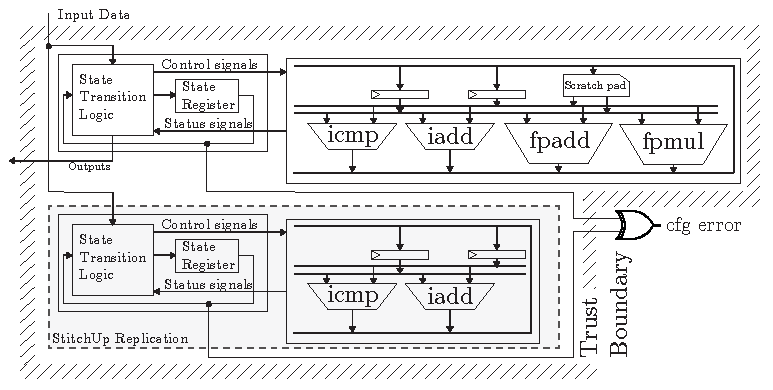
\includegraphics[width=3.5in]{./imgs/StitchUpReplication.pdf}
\caption{StitchUp Replication for the Matrix Multiplication example, with Trust Boundary}
\label{fig:HLSArch}
\end{figure}

For this paper our \emph{fault model} assumes that a single soft error
can occur at most every clock cycle, and that this error can effect block memory,
configuration memory, or flip-flops.
Since errors are not solely within the configuration memory replication must be used
over ECC/CRC codes to fully protect our control structure.
Figure \ref{fig:HLSArch} shows a StitchUp generated circuit for the matrix multiplication
example in Listing \ref{lst:MMM}, with the original circuit on top and the
control-flow structure shadow beneath it.
StitchUp aims to protect all configuration, block, and Flip-flop bits within the
trust boundary (grey box) as everything outside, such as routing to
external I/O or DDR, is not protected.


%\subsection{Error Detection and Mitigation}
%Dual Modular Redundancy (DMR) is the traditional approach for detecting faults,
%where any difference between duplicated versions of components operating with the same state indicates 
%an error.
%Typically this is performed with two identical hardware units executing in lock step and
%periodically comparing their outputs.
%
%Redundancy is often not feasible in constrained systems like satellites
%since it is inherently costly consuming area, power, time, or all of the above.
%For this reason researchers have been interested in finding methods to
%increase reliability with less redundancy but without increasing engineering effort.
%The majority of research into this problem has primarily focussed on low level approaches,
%with only a few investigations into how this can be achieved through HLS tools.
%
%The majority of modern reliable HLS work has revolved around the idea of a component
%library, where implementations of the same components with different resource to
%reliability trade offs are selected during the allocation phase of the HLS tool
%\cite{tosun2005reliability}, \cite{glass2007interactive}, \cite{hara2013cost}.
%While these works do a great job at exploring the reliability trade offs they
%all have the same assumption that reliability is equally important across
%portions of the computation, but is this necessarily true?
%
%A large number of studies within the software domain have explored the resilience of various applications
%to the injection of soft errors, and found that there are clear regions of code that
%are more critical than others LIST OF CITATIONS HERE.
%
%In \cite{wong2006soft} the authors examined probabilistic
%inference applications which are designed to be robust against noisy incomplete input
%data to see if this also translated to resilience to soft errors.
%Instruction level fault injection techniques were used to discover that such algorithms
%have a natural ability to mask multiple data errors, however control flow errors were more
%severe and tended to result in premature program termination.
%
%Within the field of approximate computing there has also been interest in separating code into
%critical and non-critical sections.
%A notable example is EnerJ \cite{sampson2011enerj} where type
%annotations indicate whether code regions should be precise or imprecise.
%The type system then ensures the segregation of imprecise code from precise code allowing for the safe execution of imprecise code on approximate hardware.
%Flikker \cite{liu2012flikker} has a similar approach where type-annotations are used to store data in
%DRAM banks that are refreshed below the recommended manufacturers rate to save idle power consumption.  
%For a selection of mobile application benchmarks they find that large portions of memory can be safely
%stored in the low refresh DRAM with minimal impact on application results.


%\subsection{Fault Model}
%
%In this work we shall focus on single \textbf{single} errors, assuming that only one SEU
%can occur per clock cycle.
%We shall also limit ourselves to SRAM based FPGA designs, although the protection scheme 
%presented in this paper can be equally applied to VLSI designs.



